%%%%%%%%%%%%%%%
%
% Compiler : GNUARM
% Installation of drivers + upload - depend on your target
%
%%%%%%%%%%%%%%%

\newpage
\section{ARM}
For ARM target, you can use GNUARM as compiler. Thus, the first section will show you how to compile gcc for ARM achitecture (you can find some binaries on GNUARM website if you prefer \href{http://www.gnuarm.com/}{http://www.gnuarm.com/}).\\
The second section depends on your board. It's the drivers installation to communicate to your board and upload a program.\\

\subsection{GNUARM}
\subparagraph{Unix}
To compile gcc for ARM architecure on UNIX system, follow all the steps below, after having download :
\begin{itemize}
\item binutils-2.19.1
\item gcc-4.4.1
\item newlib-1.17.0
\item gdb-6.8
\end{itemize}

You can download other versions of these softwares, don't forget to change the header below.\
\lstinputlisting{./install.command}

\subparagraph{Windows}
\begin{itemize}
\item Download a GCC-4.0.2 tool chain (\href{http://www.gnuarm.com/bu-2.16.1_gcc-4.0.2-c-c++_nl-1.14.0_gi-6.4.exe}{http://www.gnuarm.com/bu-2.16.1_gcc-4.0.2-c-c++_nl-1.14.0_gi-6.4.exe}).
\item Install only selected components in the below picture. ARM7(ATMEL AT91SAM7S256) in the NXT and in the Olimex board is Little Endian and does not have FPU.
\item Do not check "Install Cygwin DLLs..." because Cygwin was already installed.\\
\item At the end of the installation, you were asked about adding the tool path to Windows Environment Variables, but it would not be needed.
\end{itemize}


%%%%%%%%%%%%%%
\subsection{Board installation drivers and upload program}


\subsubsection{Lego Mindstorm NXT2.0}

%%%%%%%%%%%%%%%%%%%%%%%%%
\paragraph{Nexttool + Lego Drivers}
%%%%%%
\subparagraph{MAC OS}


Download and install the Lego Drivers (\href{http://mindstorms.lego.com/en-us/support/files/default.aspx#Driver}{http://mindstorms.lego.com/en-us/support/files/default.aspx
\#Driver}) and the firmware update (\href{http://mindstorms.lego.com/en-us/support/files/default.aspx#Firmware}{http://mindstorms.lego.com/en-us/support/files/default.aspx\#Firmware}) for MAC OS. \\
Download Nexttool (\href{http://bricxcc.sourceforge.net/utilities.html}{http://bricxcc.sourceforge.net/utilities.html}) and a new firmware (\href{http://bricxcc.sourceforge.net/lms_arm_jch.zip}{http://bricxcc.sourceforge.net/lms\_arm\_jch.zip}) and update the firmware as explained below :
\begin{itemize}
\item Reset the NXT : To go into firmware update mode, press the reset button (at the back of the NXT, upper left corner beneath the USB connector) for more than 5 seconds while the NXT is turned on. The NXT will audibly tick when it is in firmware update mode.
\item Copy an Enhanced NXT firmware (i.e. lms\_arm\_nbcnxc\_107.rfw) to NeXTTool extracted directory.
\item Launch Nexttool, and updload the Enhanced NXT firmware to the NXT (clicking on "Download firmware"), selecting it.
	\begin{figure}[h] %  figure placement: here, top, bottom, or page
   		\centering
		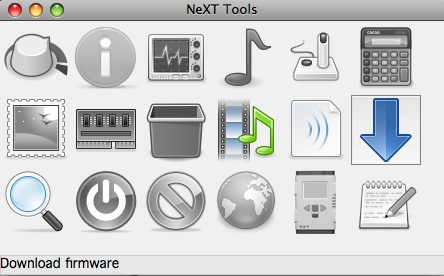
\includegraphics[width=0.7\textwidth]{pictures/firmware.jpg}
	\end{figure}
\item Remove the battery from the NXT and insert it again, and then press orange rectangle button on the NXT to turn on the Enhanced NXT firmware. The Enhanced NXT firmware has same GUI as the LEGO standard firmware.
\end{itemize}

%%%%
\subparagraph{Linux}
Note: Nextool binary for Linux seems to fail for firmware upload.\\
Install required packages:
\begin{verbatim}
$sudo apt-get install scons libusb-dev libusb-0.1-4
\end{verbatim}
Download the libnxt (\href{http://libnxt.googlecode.com/files/libnxt-0.3.tar.gz}{http://libnxt.googlecode.com/files/libnxt-0.3.tar.gz}) archive and extract it. Go in the new directory and build the project with scons:
\begin{verbatim}
$ cd libnxt-0.3/ 
$ scons
\end{verbatim}

A program call fwflash is created.\\
Download John Hansen's Enhanced NXT firmware (\href{http://bricxcc.sourceforge.net/lms_arm_jch.zip}{http://bricxcc.sourceforge.net/lms\_arm\_jch.zip}) (any version numbered 106 or later includes the native-invocation feature) and store the Enhanced NXT firmware (i.e lms\_arm\_nbcnxc\_1xx.rfw) in the directory where fwflash is stored.\\
Connect the NXT brick to usb and turn it on. Then press the reset button for more than 4s to put it in firmware upload mode (nxt display is cleared but it makes a ticking sound).\\
Flash the firmware with the following command (it takes some dozen of seconds), where 1xx is replaced by the number of the firmware:
\begin{verbatim}
$ sudo ./fwflash lms_arm_nbcnxc_1xx.rfw
\end{verbatim}

Troubleshooting: After completion of the upload, sometimes NXT display is messed and block : reboot it by a quick push on the reset button or remove the battery. If the NXT makes a ticking sound, it is still in firmware upload mode. If troubles, use and see windows firmware update procedure (and LEGO UserGuide).\\

%%%%
\subparagraph{Windows}
Download and install the Lego Drivers (\href{http://mindstorms.lego.com/en-us/support/files/default.aspx#Driver}{http://mindstorms.lego.com/en-us/support/files/default.aspx
\#Driver}) for PC. \\
Download Nexttool (\href{http://bricxcc.sourceforge.net/nexttool.zip}{http://bricxcc.sourceforge.net/nexttool.zip}) and a new firmware (\href{http://bricxcc.sourceforge.net/lms_arm_jch.zip}{http://bricxcc.sourceforge.net/lms\_arm\_jch.zip}) and update the firm-ware as explained below :
\begin{itemize}
\item Reset the NXT : To go into firmware update mode, press the reset button (at the back of the NXT, upper left corner beneath the USB connector) for more than 5 seconds while the NXT is turned on. The NXT will audibly tick when it is in firmware update mode.
\item Copy an Enhanced NXT firmware (i.e. lms\_arm\_nbcnxc\_107.rfw) to NeXTTool extracted directory.
\item Execute Cygwin and type the following command to change the current directory to the NexTTool extracted directory. (NeXTTool is assumed to be extracted under C:$\backslash$cygwin$\backslash$nexttool directory)
	\begin{verbatim}
	$cd C:\cygwin\nexttool
	\end{verbatim}
\item Connect PC and the NXT by USB cable.
\item Type the following command in Cygwin to upload the Enhanced NXT firmware to the NXT (Program upload may take around half minutes and then, NXT LCD is turned to display some chunk from blank).
	\begin{verbatim}
	$./NeXTTool.exe /COM=usb -firmware=lms\_arm\_nbcnxc\_107.rfw
	\end{verbatim}
\item Remove the battery from the NXT and insert it again, and then press orange rectangle button on the NXT to turn on the Enhanced NXT firmware. The Enhanced NXT firmware has same GUI as the LEGO standard firmware.
\end{itemize}




%%%%%%%%%%%%%%%%%%%%%%%%%
\paragraph{Upload a program}
\subparagraph{MAC OS}
To upload a program in the NXT (the nxt example examples/arm/nxt/simple/nxt\_simple\_exe.rxe)
\begin{itemize}
\item Connect the PC and the NXT by USB cable.
\item Launch Nexttool, select "usb port".
	\begin{figure}[htbp] %  figure placement: here, top, bottom, or page
   		\centering
		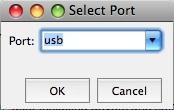
\includegraphics[width=0.25\textwidth]{pictures/usbport.jpg}
	\end{figure}
\item Go to "NXT Explorer"
	\begin{figure}[htbp] %  figure placement: here, top, bottom, or page
   		\centering
		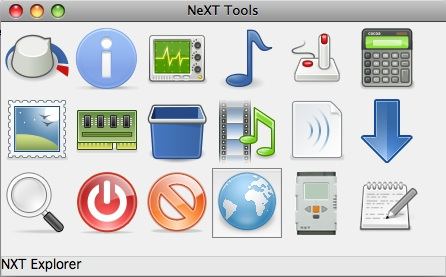
\includegraphics[width=.7\textwidth]{pictures/nxtexplorer.jpg}
	\end{figure}
\item Click on the "Download selected files to the NXT" and select the nxt\_simple\_exe.rxe file.
\item If program upload was succeeded, you can see the nxt\_simple\_exe.rxe file in the files list as below.
	\begin{center}[h] %  figure placement: here, top, bottom, or page
   		%\centering
		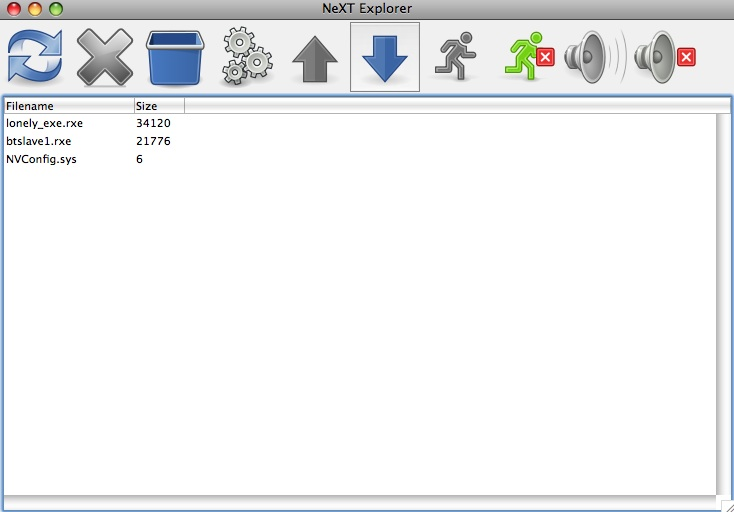
\includegraphics[width=1\textwidth]{pictures/downloadfile.jpg}
	\end{center}
\item To execute a program on the NXT, go in "My files"/"Software files".
\end{itemize}

%%%%
\subparagraph{Linux}
Required Packages: libusb-0.1-4\\
Download this executable of John Hansen's NeXTTool (\href{http://lejos-osek.sourceforge.net/installation_linux_files/NeXTTool}{here}) (built from bricxcc svn repository, revision 1)\\
Check the version of NeXTTool, it should be 1.0.1.0:
\begin{verbatim}
$ sudo ./[NEXTTOOL_PATH]/NeXTTool
nexttool version 1.0.1.0 (1.0.1.0)
Copyright (c) 2006, John Hansen
Use "NeXTTool -help" for more information.
\end{verbatim}

To ubload over usb, turn on the NXT, connect it to USB and run the following command (example: nxt\_simple\_exe.rxe) :
\begin{verbatim}
$ sudo ./[NEXTTOOL_PATH]/NeXTTool /COM=usb -download=nxt\_simple\_exe.rxe
\end{verbatim}

Troubleshooting: Test the following command to see if Nexttool is working (set execution right for NeXTTool):
\begin{verbatim}
$ sudo ./[NEXTTOOL_PATH]/NeXTTool /COM=usb -versions
Protocol version = 1.124
Firmware version = 1.xx
\end{verbatim}

To ubload over bluetooth, you need to define an alias name in a file 'nxt.dat' as explained in this post: Minsdtorm 2.0 development on linux . Then turn on the NXT and run the following command (example: nxt\_simple\_exe.rxe) :
\begin{verbatim}
$ sudo ./[NEXTTOOL_PATH]/NeXTTool /COM=alias_bt -download=nxt\_simple\_exe.rxe
\end{verbatim}

To execute a program on the NXT, go in "My files"/"Software files".

%%%%
\subparagraph{Windows}
To upload a program in the NXT (the nxt example examples/arm/nxt/lonely\_exe.rxe) follow the steps below :
\begin{itemize}
\item Connect the PC and the NXT by USB cable.
\item Type the following command in Cygwin (from examples/arm/nxt) :
	\begin{verbatim}
	$./[NEXTTOOL_PATH]/NeXTTool.exe /COM=usb -download=lonely_exe.rxe
	$./[NEXTTOOL_PATH]/NeXTTool.exe /COM=usb -listfiles=lonely_exe.rxe
	\end{verbatim}
\item If program upload was succeeded, program size could be displayed in Cygwin such as the second line in the below command outputs. 
	\begin{verbatim}
	Executing NeXTTool to upload helloworld.rxe...
	helloworld.rxe=15280
	NeXTTool is terminated.
	\end{verbatim}
\item To execute a program on the NXT, go in "My files"/"Software files".
\end{itemize}


\subsubsection{Olimex LPC-E2294}

%%%%%%%%%%%%%%%%%%%%%%%%%
\paragraph{OPENOCD + drivers}
%%%%%%
openOCD is a software that communicates via the JTAG (Open On-Chip Debug Solution for Embedded Target Systems based on the ARM7 and ARM9 Family). It's an open source software by BerliOS (http://openocd.berlios.de/web/). \\
Download and compile openOCD for your achitecture (it appears revision after 1200 are not able to compile correcty under MacOS X).\\
As you don't need just openOCD because it needs the USB driver, you've got two choice : 
\begin{itemize}
\item install libusb et libftdi
\item install D2XX
\end{itemize}

%%%%%%%%%%%%%%%%%%%%%%%%%
\paragraph{Upload a program}
To upload a program double click on \textit{2-run-openocd.command} to open the connection between your computer and the board.\\
And double click on \textit{2a-debug-external-ram.command} if you want to upload your program in external ram with debug.\\
In the debug consol type :
\begin{itemize}
\item "c" to continue
\item "b" to place a breakpoint
\item "si" to step instruction
\item "display/i \$pc" to display assembler code on the pc register
\item "x/i \$pc" to visualise the i blocs from pc
\item "info registers" to see the registers state
\end{itemize}





